% !TeX root = ../../main.tex
% Add the above to each chapter to make compiling the PDF easier in some editors.

\section{Deep Extreme Cut}\label{ord:ch3:sec3}

In \cite{Man18-DEXTR} the \gls{dextr} method for interactive segmentation is introduced.
This method follows a user point centered approach based on \gls{dl} as introduced in Subsection \ref{ord:ch2:sec3:subsec2}.

\subsection{Method Description}\label{ord:ch3:sec3:subsec1}

% Workflow
The required user interaction are four clicks in the form of extreme points.
These points are the right-most, left-most, bottom and top pixels of an object,  illustrated in Figure \ref{fig:ch3:sec3:user_interaction}.
They reflect the most extreme pixels and therefore referred to as extreme points.
The obtained user clicks are further processed and the \gls{dl} model predicts an object mask.

% Advantage over other methods
Extreme points provide a valuable guidance for the segmentation network.
First, a bounding box can easily be derived from the them.
Second, extreme points are naturally located at the object's boundary.
This provides the network with high level guidance on the localization of the boundary.
In the upsampling process this becomes especially useful, in order to reconstruct sharper borders.
% Extreme points contain more information than just a bbox
With reference to the information content, extreme points are more valuable than a bounding box.
% -> guidance for deep architectures 
% -> firhter boost accuracy of segmentation networks

\subsection{Model Input and Representation of User Clicks}\label{ord:ch3:sec3:subsec2}

The creation of the model input $\textbf{x}$ may be separated into three processing steps.

% Crop image based on bbox
First, the image is processed. 
A bounding box is derived from the extreme points. 
Further, this bounding box is enlarged by $p_{{box}}$ \Unit{px} is done to include context from the surrounding region.
% Zero Padding
If the enlarged bounding box extends the original image boundary, the overhanging pixels contain the value zero.
Manisis \etal refers to this treatment as \textit{zero padding} \cite{Man18-DEXTR}, which is illustrated at the bottom of Figure \ref{fig:ch3:sec3:user_interaction} and \ref{fig:ch3:sec3:rgb_channel}.
In order to focus on the object of interest, the image is cropped based on the enlarged bounding box and resized to the size of $512 \times 512$ \Unit{px}.

\begin{figure}
	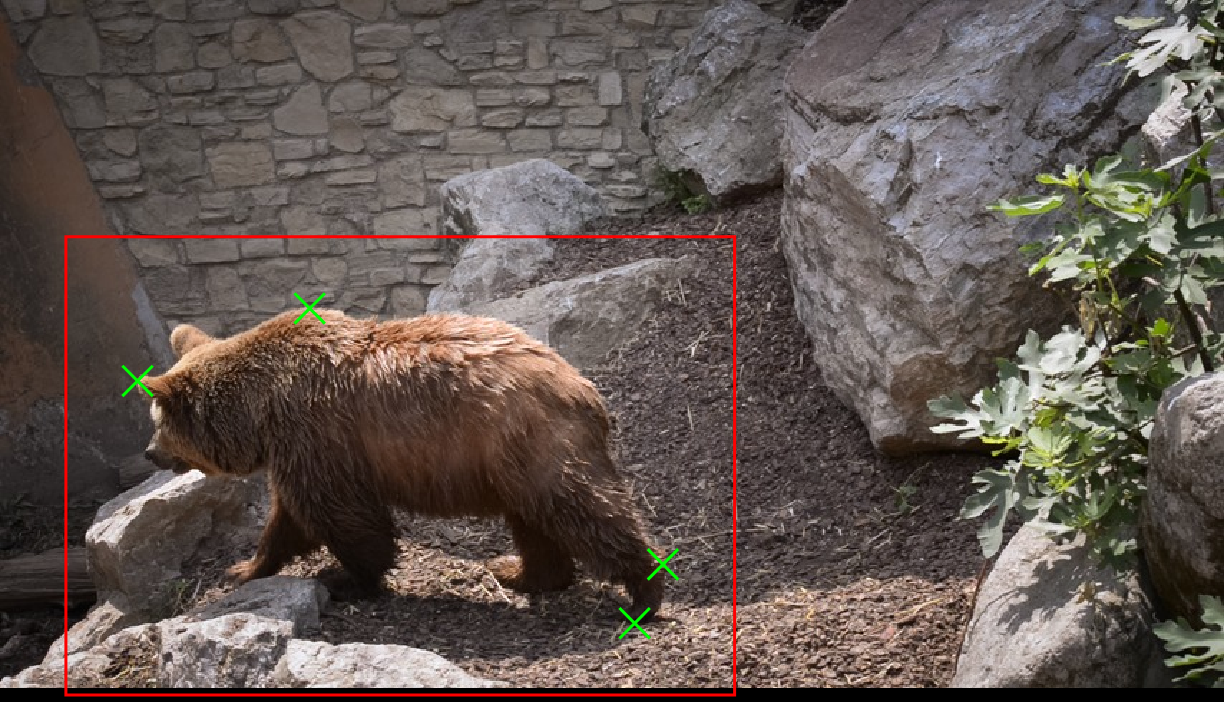
\includegraphics[width=\linewidth]{figures/chap33_bear_bbox.png}
	\caption[DEXTR User Interaction]{		
		Image with the obtained user input for the \gls{dextr} method and a first processing step.
		The extreme points are visualized as green crosses.
		The bounding box is enlarged by $p_{{box}} = 50$ \Unit{px} and shown in red.
		The enlarged bounding box extends the image boundary, therefore \textit{zero padding} is applied.
		The corresponding cropped and resized image is shown in Figure \ref{fig:ch3:sec3:rgb_channel}.
	}
	\label{fig:ch3:sec3:user_interaction}
\end{figure}


% One feature map with extreme points
Second, the four extreme points are converted into one heatmap.
This heatmap may be referred as foreground heatmap, because the extreme points are located \textit{on} the object's boundary.

To highlight the extreme points a 2D Gaussian is centered around each point by
% Impelemtation in HDevelop:
% ResGauss := exp(-4 * log(2) * ((Rows-PointRow)*(Rows-PointRow) + (Cols-PointCol)*(Cols-PointCol)) / (GaussSigma * GaussSigma))
\begin{equation} \label{equ:gauss}
	\centering
	Gauss = \frac{\exp{-4 * \log 2 }}{\sigma^{2}}
\end{equation}
with $\sigma = 10$ representing the size of the Gauss filter.
This heatmap is vital for the method, because of it's high level guidance for the deep segmentation network.
A closeup of a point centered by the 2D Gaussian is visualized in Figure \ref{fig:ch3:sec3:gauss_centered_point}.

Third, the heatmap has the size of $512 \times 512$ \Unit{px} and is concatenated with the RGB image.
This results into a four-channel \gls{dextr} model input, which is explanatory illustrated in Figure \ref{fig:ch3:sec3:model_input_channels}.

\begin{figure}
	\centering
	\begin{subfigure}[b]{0.3\textwidth}
		\centering
		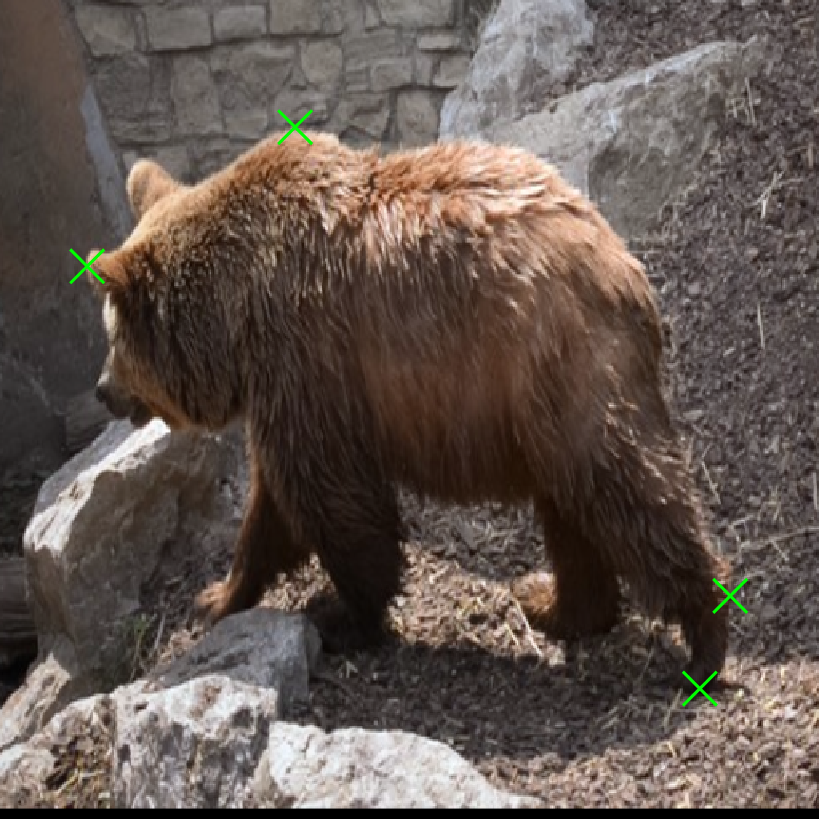
\includegraphics[width=\textwidth]{figures/chap33_channel_rgb.png}
		\caption{RGB image cropped based on the bounding box (three channels).}
		\label{fig:ch3:sec3:rgb_channel}
	\end{subfigure}
	\hfill
	\begin{subfigure}[b]{0.3\textwidth}
		\centering
		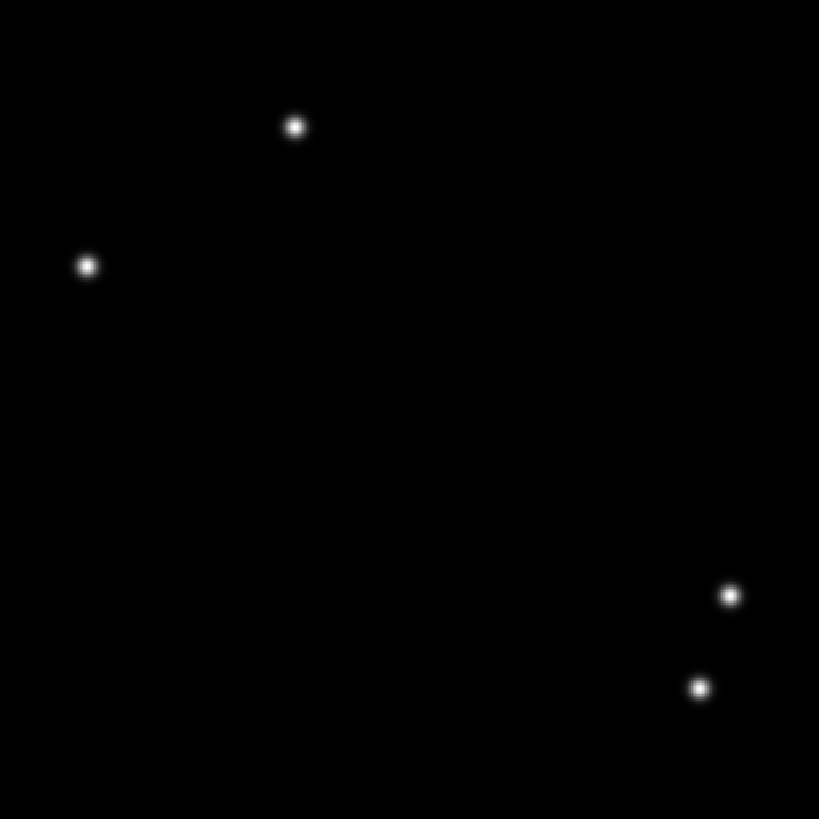
\includegraphics[width=\textwidth]{figures/chap33_channel_fg.png}
		\caption{Foreground heatmap with four extreme points (one channel).}
		\label{fig:ch3:sec3:fg_channel}
	\end{subfigure}
	\hfill
	\begin{subfigure}[b]{0.3\textwidth}
		\centering
		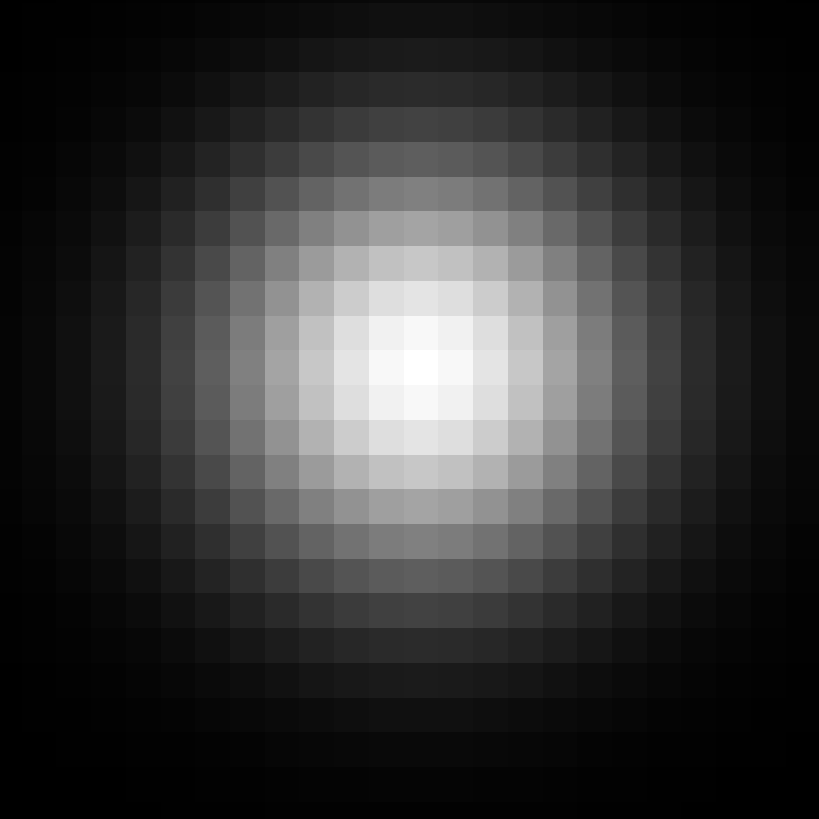
\includegraphics[width=\textwidth]{figures/chap33_gaussian_point.png}
		\caption{Closeup of a point centered with a 2D Gaussian with $\sigma = 10$.}
		\label{fig:ch3:sec3:gauss_centered_point}
	\end{subfigure}
	\caption[Four-channel DEXTR model input]{
		Representation of the separate channels from the four-channel \gls{dextr} model input.
		All channels have the spacial dimension of $512 \times 512$ \Unit{px}.
		The user points in the foreground and background are enforced with a 2D Gaussian.
	} \label{fig:ch3:sec3:model_input_channels}
\end{figure}


\subsection{Architecture}\label{ord:ch3:sec3:subsec3}

As encoder for the segmentation network \textit{ResNet-101} \cite{He16-ResNet} is selected, which if also referred to as \textit{backbone}.
The ResNet-101 is a deep \gls{cnn} containing 101 layers.
The core component of any ResNet are \textit{residual units}, that are also referred to as \textit{bottleneck block}.
Residual units contain skip connections, that are beneficial in various ways as explained in \cite{He16-ResNet} and \cite{Ger17-HandsOn}.
The ResNet-101 is structured in four blocks, that contain 3, 4, 23 and 3 residual units.

The ResNet-101 used for \gls{dextr} is modified by including atrous convolution in the last two blocks and removing the fully connected layers.

After the backbone a four staged \gls{psp} module is applied to preserve global context.
This network does not use a \textit{real} decoder, instead bilinear interpolation is used to retrieve original spatial dimension of $512 \times 512$ \Unit{px}.
In the end a sigmoid function is applied to obtain the final prediction $y$ as a  probability map.
% TODO footnote for sigmoid fucntion.
% Special thing about this network is the basically missing decoder and skip connections over the network -> that shows how valuable the border-click information is?

\subsection{Refinement}\label{ord:ch3:sec3:subsec4}

As introduced in Subsection \ref{ord:ch2:sec3:subsec2}, some interactive methods provide the possibility to perform refinement, if a segmentation result does not meet the user's expectations.
For the \gls{dextr} method the user may perform refinement by setting an additional click.
The refinement click should be located on the boundary of the region where the segmentation fails.
This new refinement click is added to the foreground heatmap with the extreme points.
In Figure \ref{fig:ch3:sec3:refinement} the effect of an additional refinement click is exemplary presented.
Each refinement clicks triggers a new model execution.
The refinement process may be applied iteratively.

% TODO use an example where the initial prediction actually fails and the refinement succeeds.
\begin{figure} 
	\centering
	\begin{subfigure}[b]{0.45\textwidth}
		\centering
		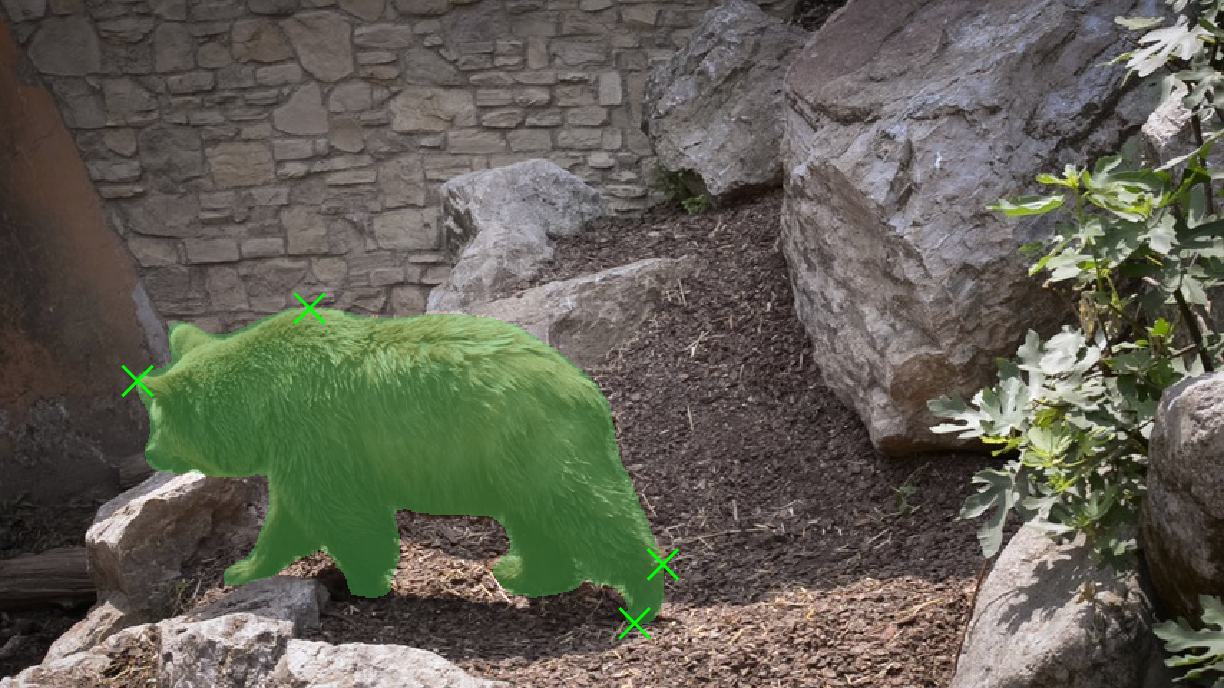
\includegraphics[width=\textwidth]{figures/chap33_bear_initial_result.png}
		\caption{Initial segmentation result.}
		\label{fig:ch3:sec3:refinement_1}
	\end{subfigure}
	\hfill
	\begin{subfigure}[b]{0.45\textwidth}
		\centering
		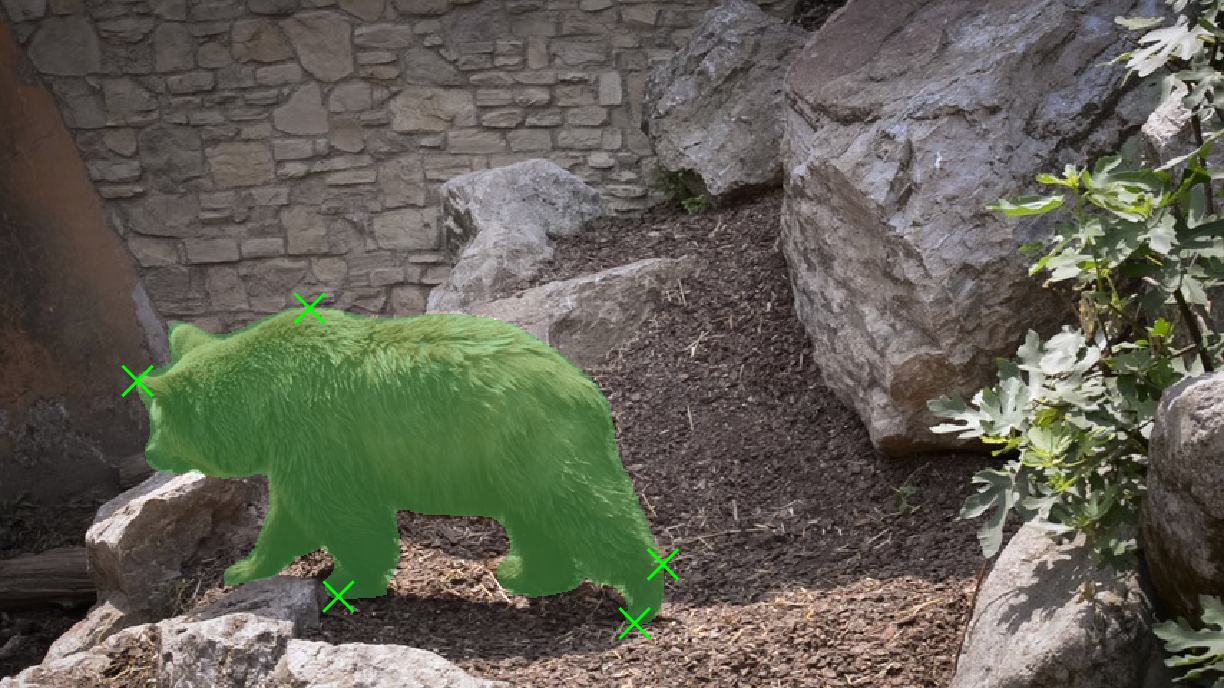
\includegraphics[width=\textwidth]{figures/chap33_bear_refine_result.png}
		\caption{Refinement segmentation result.}
		\label{fig:ch3:sec3:refinement_2}
	\end{subfigure}
	\caption[DEXTR Refinement]{
		On the left is the initial result with the normal extreme points. 
		On the right is the segmentation result with one additional refinement click.
	} \label{fig:ch3:sec3:refinement}
\end{figure}


\subsection{Performance}\label{ord:ch3:sec3:subsec5}

The performance of the \gls{dextr} method in comparison to other interactive segmentation methods in shown in Table \ref{tab:ch2:interactive-stae-of-the-art}.
In this comparison on Pascal VOC the \gls{dextr} method performs well and is only outperformed by the \gls{iog} method.

The experiments and evaluations presented in \cite{Man18-DEXTR} contain various datasets and test settings.
Among them is also an examination of the performance on unseen classes and the method's generalization capability.
Thereby, the model was trained with the Pascal VOC or COCO dataset and evaluated on both datasets.
Despite these results seem reliable, it must be taken into account that the Pascal VOC and COCO datasets are very similar and cover the same type of \textit{general} objects.
The evaluation of the network's generalization capabilities is continues in detail in Chapter XXX.
% TODO ref chapter  section.

An introduced application for the \gls{dextr} method is to create annotations and use them as new \gls{gt} to train \gls{dl} models.
Manisis \etal claim, that models trained on \gls{dextr} annotations perform equally well as models trained on the original \gls{gt}\cite{Man18-DEXTR}.
This statement is further examined in Section XXX.
% TODO ref section with RE-1470.